\chapter{Integration of Transfer Learning}\label{In}
In this chapter, two versions of the \ac{PCTKVM} are proposed.
The \acs{PCTKVM} which handles the $\theta$ as fixed parameter and the \acs{PCTKVM}\textsubscript{$\theta$Est}, which does a theta estimation.
The extensions 'TK' to original term \acs{PCVM} should indicate the new Kernel approach to solve the transfer learning problem.
As already mentioned in \ref{Tl} there are various solutions to solve the transfer learning problem.
Revisiting section \ref{TlSecHomo}, the homogeneous transfer learning problem can be summarised in four approaches.\newline
However, Long et al. in \cite{Long.2015} proposed a different approach, which differs from the approaches and therefore called it transfer kernel learning.
However, because the relational knowledge approach transfers information through defined relationships between the source and target data, from section \ref{TlSubSecRelation}, the \acs{TKL} suits well in this category.
Furthermore, because it needs target data for the learning process and according to the definition of transductive transfer learning from section \ref{TlSubSecTrans}, it can be categorised as transductive transfer setting.\\
The main idea of it is to approximate the kernel of the training set with the kernel of the test set via the Nyström kernel approximation.\cite{Long.2015}
On the other side \cite{Schleif.2015}, proposed a \acs{PCVM} with linear costs which is also achieved via the Nyström approximation.
Therefore it seems reasonable to go one step further an combine these two ideas to form a transfer learning \acs{PCVM}.\\
Another advantage is that \acs{TKL} is very simple when it comes to dataset usage.
According to \ref{TlSecDef} there are transfer learning solutions which need prelabeled test data.
As we will see in the following the \acs{TKL} using only the training and test dataset as it is to compute the transfer kernel and therefore has an 'easy' handling.\newline
However, before going into the approach itself, the underlying technique should be discussed.
See section \ref{EmSubSecKernel} for details to kernels and the Gram matrix.
\section{Nyström Approximation}\label{InSecNysMeth}
The main Problem by computing eigenvalues and eigenvectors is that optimal eigenvalue decomposition has a time complexity of $\mathcal{O}(N)^3$ and alternative approaches must be found.
The Nyström Method was originally made for solving the eigenvalue equation, which can be seen in equation \eqref{EqEigsEq}.\cite{Zhang.2008}\\
It is done by selecting $N$ randomly observations (rows/columns) without replacement of $\mathbf{K}$ for calculating the approximation.\cite{Williams.2000}
Considering a symmetric positive semi definite kernel $k(\mathbf{z},\mathbf{x})$ which satisfies Mercers Theorem, then $K$ has the following properties and can be represented as:\cite{Williams.2000}
\begin{equation}\label{EqKernelRep}
	k(\mathbf{z},\mathbf{x}) = \sum_{i=1}^{N}\lambda_i\phi_i(\mathbf{z})\phi_i(\mathbf{x}) 
\end{equation}
With $N < \infty$ as the number of feature space dimensions and $\lambda_1 \ge \lambda_2\ge\dots\ge0$ as the sorted eigenvalues and $\phi_i$ as eigenfunctions.
As consequence of Mercer follows that  $\lambda_i$ and $\phi_i$ have to satisfy the eigenvalue equations:
 \begin{equation}\label{EqEigsEq}
	\int_{i=1}^{N} k(\mathbf{x},\mathbf{z})\phi_i(\mathbf{z})p(\mathbf{z})d\mathbf{x} = \lambda_i\phi_i(\mathbf{x})
\end{equation}
With $p(z)$ as the probability density of the input vector $\mathbf{z}$.
Furthermore, the orthogonality conditions are satisfied with:\cite[p. 59]{Scholkopf.2001}
\begin{equation}\label{EqEigsOrt}
	\int \phi_i(\mathbf{z})\phi_j(\mathbf{z})p(\mathbf{z})d\mathbf{z} = \delta
\end{equation}
If a kernel defined above is given, then an empirical estimate can be done by, drawing an identical and independently sample ${\mathbf{z}_1,\dots,z_q}$ from $p(\mathbf{z})$.
The integral can be rewritten as an empirical estimate:\cite{Williams.2000}
\begin{equation}\label{EqEigsEmp}
	\sum_{k=1}^{N}\frac{k(\mathbf{x},\mathbf{z}_k)\phi_i(\mathbf{z}_k)}{N} \approx \lambda_i\phi_i(\mathbf{x})
\end{equation}
Where $N$ are the number of used observation from the kernel and the $N$ eigenfunctions are still orthogonal.
If we consider the N columns from $\mathbf{K}$ as separate kernel matrix $\mathbf{K}^{(N)}$ with size $N\times N$ and elements $K_{ij}^{(N)}=K(\mathbf{z_i,z_j})$ for $i,j=1,\dots,N$, then we can use this for the eigenvalue problem of this kernel:\cite{Williams.2000}
\begin{equation}\label{EqEigsProb}
	\mathbf{K}^{(N)}\mathbf{U}^{(N)} = \mathbf{U}^{(N)}\mathbf{\Lambda}^{(N)}
\end{equation} 
With $\mathbf{U}^{(N)} \in \mathbb{R}^{N\times N}$ as eigenvectors and $\boldsymbol{\Lambda}^{(N)}$ as diagonal matrix with the eigenvalues for the small kernel with $\lambda_1^{(N)}\ge\lambda_2^{(N)}\ge\dots\lambda_N^{(N)} \ge0$.
If we consider points within the kernel $K^{(N)}$, then $\mathbf{x}$ can be replaced with $\mathbf{z}_j$.
Furthermore, matching \eqref{EqEigsProb} against \eqref{EqEigsEmp} then the following approximation can be obtained:\cite{Williams.2000}
\begin{equation}\label{EqEigsFuncAprox}
	\phi_i(\mathbf{z}_j) \approx \sqrt{q}U_{ij}^{(N)}
\end{equation}
Finally, by using $\phi_i(x_k)$ in \eqref{EqEigsEmp} the approximation for the any eigenvector or eigenvalues can be given by:
\begin{equation}\label{EqEigsValAprox}
	\phi_i(\mathbf{x})\approx\frac{\sqrt{q}}{\lambda_i^{(N)}}\sum_{k=1}^{N}k(\mathbf{x},\mathbf{z_k})U_{k,i}^{(N)}, \>\>\>\>\> \lambda_i \approx \frac{\lambda_i^{(N)}}{q}
\end{equation}
With this the $i$-th eigenfunctions and eigenvalues can be approximated by calculating the sample kernel.\cite{Williams.2000}
As a consequence the eigenfunctions and eigenvalues of the whole kernel can be approximated.
\subsection{Nyström Kernel Learning}\label{InSubSecNyKerneLearning}
Willams and Seeger extended the work of Nyström to speed up kernel machines.
The problem with kernel-based predictors, e.\,g. \acs{SVM}, is similar to the eigenvalue decomposition problem from section \ref{InSecNysMeth}
It requires the computational complexity of $\mathcal{O}(N^3$), with $N$ as the number of training examples, to find a solution.\cite{Williams.2000}\\
With the Nyström approximation the complexity for predictors can be bound by $\mathcal{O}(M^3N)$ with using a smaller system with size $M$, where $M<N$.\cite{Williams.2000}\\	
Now the goal is to create a low-rank approximation Matrix $\tilde{\mathbf{K}}$ of the original $N\times N$ kernel matrix $\mathbf{K}$.
Revisiting section \ref{InSecNysMeth}, using the technique of Nyström, a kernel $\mathbf{K}$ which satisfies Mercers theorem is needed.\cite{Williams.2000}
Furthermore, we draw $M$ \acs{IID} samples of $\mathbf{K}$ and therefore we can rewrite the symmetric kernel according to:\cite{Nemtsov.2016}
\begin{equation}\label{EqNystKernelParts}
	\mathbf{K} = 
	\begin{bmatrix}
		 \mathbf{K}_{M,M}\>\>\>\> \mathbf{K}_{M,N-M} \\
		 \mathbf{K}_{N-M,M}\>\>\>\> \mathbf{K}_{N-M,N-M}
	\end{bmatrix}
\end{equation}
Where $\mathbf{K}_{M,M}$ is the sample matrix and $\mathbf{K}_{N-M,M}$ is the submatrix of $\mathbf{K}$, which is the kernel of the sample, and the rest of the data $\mathbf{K}_{N-M,N-M}$.
Because $\mathbf{K}$ is symmetric $\mathbf{K}_{N-M,M} = (\mathbf{K}_{M,N-M})^T$.
Furthermore, $\mathbf{K}_{N-M,N-M}$ is the part of the kernel which is not sampled or 'used' for the approximation, as we will see.\\
Motivated from the general eigenvalue problem, which can obtained from \cite[p. 221]{Hartmann.2015} and shown in \eqref{EqEigsProb}, a kernel can be calculated with $\tilde{\mathbf{K}} = \tilde{\mathbf{U}}\tilde{\mathbf{\Lambda}}\tilde{\mathbf{U}}^T=\sum_{i=1}^{p}\tilde{\lambda}_i^{(N)}\tilde{\mathbf{u}}_i^{(N)}(\tilde{\mathbf{u}}_i^{(N)})^T$ and is in this case the approximation matrix.\cite{Williams.2000}
With the approximated eigenvalues and eigenvectors as $\tilde{\lambda}_i^{(N)}$ and $\tilde{\mathbf{u}}_i^{(N)}$ respectively.\\
Therefore, we proceed with the equations to approximate the eigenvalues and eigenvectors.
By choosing $P\le M<N$  as the size of the subset and applying the equations of \eqref{EqEigsFuncAprox} and \eqref{EqEigsValAprox}, the approximation bases on the approximation sample matrix can be made with:\cite{Zhang.2008}
\begin{equation}\label{EqNystEigsApprox}
	\begin{gathered}
			\tilde{\lambda}_i^{(N)} = \frac{N}{M}\lambda_i^{(M)} \>\>\>\>\> \sim \>\>\>\>\> \boldsymbol{\Lambda}^{(N)} =\frac{N}{M}\boldsymbol{\Lambda}^{(M)}\\
			\tilde{\mathbf{u}}_i^{(N)} = \sqrt{\frac{M}{N}}\frac{1}{\lambda_i^{(M)}}\mathbf{K}_{N,M}\mathbf{u}_i^{(M)}\>\>\>\>\> \sim \>\>\>\>\> \mathbf{U}^{(N)} = \sqrt{\frac{M}{N}}\mathbf{K}_{N,M}\mathbf{U}^{(M)}(\boldsymbol{\Lambda}^{(N)})^T
	\end{gathered}
\end{equation}
With $i=1,\dots,P$ and $u_i^{(M)}$ and $\lambda_i^{(M)}$ from the eigenproblem and from the $M\times M$ sample kernel $K_{M,M}$.\\
After obtaining the approximated eigenvalues and vectors the full approximated kernel can be restored:\cite{Williams.2000}\cite{Zhang.2008}
\begin{equation}\label{EqNystKernelEigsApprox}
	\tilde{\mathbf{K}} = \bigg(\sqrt{\frac{M}{N}}\mathbf{K}_{N,M}\mathbf{U}^{(M)}(\boldsymbol{\Lambda}^{(N)})\bigg)\bigg(\frac{N}{M}\boldsymbol{\Lambda}^{(M)}\bigg)\bigg(\sqrt{\frac{M}{N}}\mathbf{K}_{N,M}\mathbf{U}^{(M)}(\boldsymbol{\Lambda}^{(N)})\bigg)^T 
\end{equation}
With the use of $\tilde{\mathbf{K}} = \tilde{\mathbf{U}}\tilde{\mathbf{\Lambda}}\tilde{\mathbf{U}}^T$ in equation \eqref{EqNystEigsApprox} the approximation can be rewritten as:
\begin{equation}\label{EqNystKernelApprox}
		\tilde{\mathbf{K}} = \mathbf{K}_{N,M}(\mathbf{K}_{M,M})^{-1}\mathbf{K}_{M,N}
\end{equation}
From \eqref{EqNystKernelApprox} can be seen that the kernel approximation can fully be done by the sample matrix and the submatrix $K_{N-M, N}$ of the 'original' kernel.\cite{Williams.2000}\\
The Nyström Kernel approximation is bounded by the error  $E_{Nys}=||\mathbf{K}-\tilde{\mathbf{K}}||$.\cite{He.2017}
This error can be minimised by choosing the samples carefully and a reasonable amount of it.
If the original Kernel $\mathbf{K}$ has to rank $M$ and the samples are linearly independent columns from the kernel, then the approximation is exact.
As a consequence from above choosing $P< M$ the error rises the fewer columns are chosen.\cite{Williams.2000}\\
The problem with choosing (sampling) columns/rows is that we usually do not know which columns are linearly independent.
May, therefore, some sampling methods or approximations are made in the past to make this sampling more deterministic.
For example, \cite{Kumar.2012}, which tries to find good samples through various sampling techniques, or \cite{Li.2015}, where the authors are drawing a large sample but approximate the submatrices with \ac{SVD}.\\
To summarise the Nyström Kernel approximation, first, we select $P$ of $N$ 'good' samples from the data reorganising the kernel according to \eqref{EqNystKernelParts}
At this point, we have two options.
First calculating the kernel just for the $\mathbf{K}_{P, P}$ and the submatrix $\mathbf{K_{N-P, P}}$, continuing with approximate the eigenvectors and eigenvalues and finally calculating the approximated kernel $\tilde{\mathbf{K}}$ \eqref{EqNystKernelEigsApprox}.
Second Calculate the approximation directly from the kernel as shown in \ref{EqNystKernelApprox}.
Note that the second one needs a matrix inversion, which should be reflected when it comes to for large datasets.

\section{Domain Invariant Kernel Learning}\label{InSecTrans}
The \ac{TKL} approach is made by Long et al. in  \cite{Long.2015}\footnote{http://ise.thss.tsinghua.edu.cn/~mlong/doc/transfer-kernel-learning-tkde15.zip}.
They are interpreting the kernel approximation from a different viewpoint.
The main idea is to see the train dataset-matrix, which has to be approximated, regarding Nyström, which will be approximated by the test dataset. Proceed by finding eigenvalues in a way that the difference between the approximation and ground truth train kernel will be minimal. This forms a domain invariant kernel for transfer learning.\cite{Long.2015}
The main Process is shown in figure \ref{FigTKLApp}.\newline 
From the above consider $\mathbf{z}$ as $\mathbf{Z}=\{\mathbf{z}_1,\dots,\mathbf{z}_{N_\mathcal{Z}}\}$ as training dataset which is sampled from $p(\mathbf{Z})$ within training domain $\mathcal{Z}$ and $\mathbf{x}$ as $\mathbf{X}=\{\mathbf{x}_1,\dots,\mathbf{x}_{N_\mathcal{X}}\}$ as test dataset sampled from $p(\mathbf{X})$ within the test domain $\mathcal{X}$.
The definitions are based on \ref{TlSecDef}.
The associated kernels are $\mathbf{K}_\mathcal{Z}$ for training and $\mathbf{K}_\mathcal{X}$ for testing.\\
As fundamental insight of the \acs{RKHS} is that any \ac{PSD} kernel can be reconstructed based on the eigensystem of it. Furthermore any new datasets can be incorporated within a kernel.\cite{Long.2015}\\
This means given a kernel $\mathbf{K}_\mathcal{X}$ of the dataset, using only the eigensystem $\{\lambda_i,\phi_i(\mathbf{x})\}$ the kernel can be evaluated by any new data point $\mathbf{z}$ and finally generating the kernel $\mathbf{K}_\mathcal{Z}$.
Again we could approximate the needed training kernel through:\cite{Long.2015}
\begin{equation}\label{EqTrainTestApprox}
	\mathbf{K}_\mathcal{Z} \simeq \mathbf{U}_\mathcal{Z}\boldsymbol{\Lambda}_\mathcal{X} \mathbf{U}_\mathcal{Z}^T = \mathbf{K}_\mathcal{ZX}\mathbf{K}_\mathcal{X}^{-1}\mathbf{K}_\mathcal{XZ}
\end{equation}
Where $\mathbf{U}_\mathcal{Z}$ as eigenvectors of the training kernel, $\boldsymbol{\Lambda}_\mathcal{X}$ as eigenvalues of the target kernel and $\mathbf{K}_\mathcal{ZX} = \mathbf{K}_\mathcal{ZX}^T$.
This is, in fact, a rewritten version of \eqref{EqNystKernelApprox}.\\
However, there might be a major problem.
Regarding two feature spaces, especially when it comes to transfer learning, where we have taken in section \ref{TlSecDef} the assumption that test and training feature spaces following different probability distributions.
This means that $P(\mathbf{z})\neq P(\mathbf{z})$, the error of the approximation from \eqref{EqTrainTestApprox} can be arbitrary large.\cite{Long.2015}\\
However, to align the distribution difference is one goal of transfer learning.
The main improvement done by Long et al. is to tackle this problem and to learn the domain invariant approximated kernel $\mathbf{\expP{K}}_{\mathcal{A}}$.\cite{Long.2015}
\begin{figure}
	\centering
	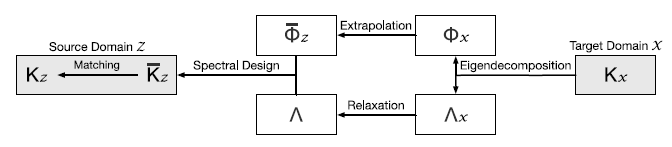
\includegraphics[width=.8\linewidth]{figures/ProcessTKL.png}
	\caption[Tranfer Kernel Learning Process]{The Process of the Domain Invariant Kernel learning.\cite{Long.2015}}
	\label{FigTKLApp}
\end{figure}
\subsection{Learning Approach}\label{InSubSecLearnApp}
From a 'kernel' viewpoint the aligning distribution of data, where the kernel is base on, can be formulated as $P(\phi(\mathbf{z})) \simeq P(\phi(\mathbf{x}))$.\cite{Long.2015}
However, handling the data distribution in Hilbert space is difficult, because the kernel-induced feature map cannot be explicitly represented.\cite{KaiZhang.2013}\\
Therefore Long et al. take the assumption that it is sufficient that $\mathbf{K}_\mathcal{Z} \simeq \mathbf{K}_\mathcal{X}$.
However, there is another problem coming up with it, because it can not be assumed that the training and test sets are equal, which means that the size of the kernels is not equal, i.\,g. $\mathbf{K}_\mathcal{Z} \in \mathbb{R}^{N_\mathcal{Z}\times N_\mathcal{Z}}$ and $\mathbf{K}_\mathcal{X} \in \mathbb{R}^{N_\mathcal{X}\times N_\mathcal{X}}$ with $N_\mathcal{Z} \neq N_\mathcal{X}$.
Therefore the extrapolated source kernel $\expP{\mathbf{K}}_\mathcal{Z} \in \mathbb{R}^{N_\mathcal{Z}\times N_\mathcal{Z}}$, by using the eigensystem of the target kernel $\mathbf{K}_\mathcal{X}$. The kernel  $\expP{\mathbf{K}}_\mathcal{Z} $ will be compared to the actual training kernel $\mathbf{K}_\mathcal{Z}$.\cite{Long.2015}\\
For clarity the terms, Long et al. proposed the term extrapolated instead of approximation.\cite{Long.2015}
In this thesis, we will stick to the proposed notation to coincide.\\
The task is now to learn this extrapolated kernel, which is done step by step by first \textit{extrapolate} the eigenvectors with:\cite{Long.2015}
\begin{equation}\label{EqExtraEigs}
	\expP{\mathbf{U}}_\mathcal{Z} \simeq \mathbf{K}_\mathcal{ZX}\mathbf{U}_\mathcal{X} \boldsymbol{\Lambda}_\mathcal{X}^{-1}
\end{equation}
According to Nyström, the eigenvalues $\boldsymbol{\Lambda}_\mathcal{X}$ of the test kernel are indispensable.
However, in this approach a \textit{relaxation} of the eigenvalues is done by considering the eigenvalues as learnable parameters $\boldsymbol{\Lambda} = diag[\lambda_1,\dots,\lambda_{N_\mathcal{X}}]$.
Therefore the kernel extrapolation can be expressed as:\cite{Long.2015}
\begin{equation}
	\expP{\mathbf{K}}_\mathcal{Z} = \expP{\mathbf{U}}_\mathcal{Z} \boldsymbol{\Lambda} \expP{\mathbf{U}}_\mathcal{Z}^T
\end{equation}
With that $\boldsymbol{\Lambda}$ does not necessarily reduce the distribution difference and has to be well chosen.
This approach should preserve the original structure of the test domain while remaining flexible to solve the difference in distribution.
Another viewpoint is that the kernel is extrapolated from the target data but evaluated by the training data.\cite{Long.2015}\\
To construct the new kernel, Long et al. using the key knowledge from spectral kernel design:
It states that a kernel which is generated from the eigensystem of another positive definite kernel, then the produced kernel will positive semi-definite itself.\cite{KaiZhang.2013}.
In general kernel matrices which are positive semi-definite have only non-negative eigenvalues.\cite[p. 30]{Scholkopf.2001}\\
Therefore it seems reasonable to set $\lambda \ge 0$ to guarantee a \acs{PSD} kernel.
The error of the approximation $\expP{\mathbf{K}}_\mathcal{Z}$ to the original ground truth kernel $\mathbf{K}_\mathcal{Z}$ is determined using the squared loss, which is presented in the following:\cite{Long.2015}
\begin{equation}\label{EqTKLSquareErrorLoss}
	\begin{gathered}
		\min_{\boldsymbol{\Lambda}} || \expP{\mathbf{K}}_\mathcal{Z} - \mathbf{K}_\mathcal{Z}||^2_F = || \expP{\mathbf{U}}_\mathcal{Z} \boldsymbol{\Lambda}  \expP{\mathbf{U}}_\mathcal{Z}^T - \mathbf{K}_\mathcal{Z} ||^2_F \\
		\lambda_i \ge \zeta \lambda_{i+1}, i = 1,\dots,N_\mathcal{X}-1 \\
		\lambda_i \ge 0,  i = 0,\dots,N_\mathcal{X}
	\end{gathered}
\end{equation}
With $\zeta \ge 1$ is the eigenspectrum dumping factor since the eigenspectrum is power law distributed and therefore $\zeta$ should produce larger eigenvectors.
With this they should contribute more to the knowledge process.\cite{Long.2015}
\subsection{Learning Algorithm}\label{InSubSecLearnAlgo}
In the above section, we defined the squared error loss function for the \acs{TKL} approach.
In this subsection, we will introduce the resulting optimisation problem and the \acs{TKL} algorithm in general.\\
The learning problem is convex and therefore will always find the global minimum.
Furthermore, it is a \ac{QP} with linear constrains which can be solved for example by the build in Matlab package \textit{quadprog}.
The squared loss function from \eqref{EqTKLSquareErrorLoss} is reformulated in a general matrix format and is expressed as:\cite{Long.}
\begin{equation}\label{EqTklQP}
	\begin{gathered}
		\min_{\boldsymbol{\lambda}} \boldsymbol{\lambda}^T \mathbf{Q} \boldsymbol{\lambda} - 2\mathbf{r}^T\boldsymbol{\lambda}\\
		\mathbf{C}\boldsymbol{\lambda} \ge 0 \\
		\boldsymbol{\lambda} \ge 0 \\
	\end{gathered}
\end{equation}
The inequalities representing the linear constrains.
The coefficient matrix $\mathbf{Q}$, $r$ and the constraint matrix C are defined as:
\begin{equation}\label{EqTklQPCons}
		\begin{gathered}
			\mathbf{Q} = (\expP{\mathbf{U}}_\mathcal{Z} \expP{\mathbf{U}}_\mathcal{Z}^T)\odot (\expP{\mathbf{U}}_\mathcal{Z}^T \expP{\mathbf{U}}_\mathcal{Z})\\
			r = diag[\expP{\mathbf{U}}_\mathcal{Z}^T \mathbf{K}_\mathcal{Z} \expP{\mathbf{U}}_\mathcal{Z}]\\
			\mathbf{C} = \mathbf{I} - \zeta \mathbf{I}
		\end{gathered}
\end{equation}
Where $\mathbf{I} \in \mathbb{R}^{N_\mathcal{X}\times N_\mathcal{X}}$ as the identity matrix and $\odot$ as hardamatrix multiplication.
Note that the eigenspectrum dumping factor $\zeta$ is the only free parameter which needs to be tuned because the $\boldsymbol{\Lambda}$ is learned within the optimisation problem.\\
Finally, similar to equation \ref{EqNystKernelParts}, we can reconstruct the 'joint' Kernel:\cite{Long.}
\begin{equation}\label{EqTKLKernel}
	\expP{\mathbf{K}}_\mathcal{A} = 
	\begin{bmatrix}
	 \expP{\mathbf{U}}_\mathcal{Z} \boldsymbol{\Lambda} \expP{\mathbf{U}}_\mathcal{Z}^T \>\>\>\> \expP{\mathbf{U}}_\mathcal{Z} \boldsymbol{\Lambda} \mathbf{U}_\mathcal{X}^T \\
	 \mathbf{U}_\mathcal{X} \boldsymbol{\Lambda} \expP{\mathbf{U}}_\mathcal{Z}^T \>\>\>\> \mathbf{U}_\mathcal{X} \boldsymbol{\Lambda} \mathbf{U}_\mathcal{X}^T 
	\end{bmatrix}
	= 	 \expP{\mathbf{U}}_\mathcal{A} \boldsymbol{\Lambda} \expP{\mathbf{U}}_\mathcal{A}^T 
\end{equation}
Where $\mathcal{A}= \mathcal{Z} \cup \mathcal{X}$ as one dataset and therefore it forms the matrix $ \expP{\mathbf{U}}_\mathcal{A} =[ \expP{\mathbf{U}}_\mathcal{A};\>  \mathbf{U}_\mathcal{X}]$, which are the extrapolated eigenvectors of the whole dataset.\newline
The complete \acs{TKL} algorithm is summarized in algorithm \ref{PseudoCodeTKL}.\cite{Long.2015}
\begin{algorithm}
	\caption{Transfer Kernel Learning Algorithm}\label{PseudoCodeTKL}	
	\begin{algorithmic}[1]
		\Require Input Data $\mathbf{I} = [\mathbf{Z};\mathbf{X}]$; kernel(-type) $k$; eigenspectrum dumping factor $\zeta$.
		\Ensure Domain invariant kernel $\expP{\mathbf{K}}_\mathcal{A}$.
		\State Compute the kernel parts $\mathbf{K}_\mathcal{Z}$, $\mathbf{K}_\mathcal{X}$ and $\mathbf{K}_\mathcal{ZX}$ with $k$.
		\State Eigendecompose of $\mathbf{K}_\mathcal{X}$ for $\{\mathbf{\Lambda}_\mathcal{X}, \mathbf{U}_\mathcal{X}\}$ like \eqref{EqEigsProb}.
		\State Extrapolate for source eigensystem  $\expP{\mathbf{U}}_\mathcal{Z}$ with \eqref{EqExtraEigs}.
		\State Solve the \acs{QP} for eigenspectrum $\mathbf{\Lambda}$ with \eqref{EqTklQP}.
		\State Merge results and return it as \eqref{EqTKLKernel}.
	\end{algorithmic}
\end{algorithm}
The underlying kernel which is calculated in the first row of algorithm \ref{PseudoCodeTKL} is the Gaussian Kernel from \eqref{EqRBFAKernel}.\\
The error of the approximation of the \acl{TKL} algorithm is $E_{TKL} = \Vert \expP{\mathbf{U}}_\mathcal{Z} \boldsymbol{\Lambda}\expP{\mathbf{U}}_\mathcal{Z}^T - \mathbf{K}_\mathcal{Z}\Vert$.
Furthermore, the approximation error of the Nyström kernel is bound by $E_{NystKer} = \Vert \mathbf{K}_{\mathcal{ZX}} \mathbf{K}_{\mathcal{X}}^{-1}\mathbf{K}_{\mathcal{XZ}}\Vert$.
Based on this errors, if $\boldsymbol{\Lambda} = \boldsymbol{\Lambda}_\mathcal{X}$, then the errors of $E_{NystKer}$ and $E_{TKL}$ are equal. 
However, because the $\boldsymbol{\Lambda}$ is a free parameter and the approximation error is directly minimised, the error of the \acs{TKL} approximation is bound by $E_{TKL}\le E_{NystKer}$.\cite{Long.}\\
In many real-world problems, the eigenvalues are following the power law distribution.
This means that there a few large eigenvalues and many small, in comparison with the large, eigenvalues.\cite{Mihail.2002}
Therefore it is considered as unnecessary to use the whole eigenspectrum and just compute the $R$ largest eigenvalues.
This is used to speed up the computation because the problem is greatly reduced.
The amount of eigenvectors is therefore fixed to $R=min(500,N_\mathcal{X})$ and therefore the eigenvectors can be reduced to $\expP{\mathbf{U}}_\mathcal{Z} \in \mathbb{R}^{R\times R}$ or $\mathbf{\lambda} \in \mathbb{R}^{R\times N_\mathcal{X}}$.\cite{Long.}\\
The complexity of the \acs{TKL} algorithm can be given with $\mathcal{O}((D+R)(N_\mathcal{Z}+N_\mathcal{X})^2)$, where $R$ denotes the number of used eigenvectors, $D$ refers to the kernel.\cite{Long.}
\section{PCTKVM Algorithm}\label{InSecAlgo}
In this section the \acl{PCTKVM} algorithm will be discussed in detail.
As shown above we have obtained our transfer learning kernel with algorithm \ref{PseudoCodeTKL}.
According to \cite{Long.2015} the new kernel can be feed to any kernel machine.
This means that we can train the regular \acf{PCVM} with our new kernel.
To train it we are using the extrapolated training kernel which is.
\begin{equation}
	\expP{\mathbf{K}}_\mathcal{Z} = \expP{\mathbf{U}}_\mathcal{Z}\mathbf{\Lambda}\expP{\mathbf{U}}_\mathcal{Z}^T
\end{equation}
However, simply using it in algorithm \ref{PseudoCodePcvm} has some disadvantages.
Revisiting the \acs{PCVM} algorithm the kernel is recalculated in every iteration based on the optimised theta from the previous iteration.
As a consequence, we have to recalculate the entire transfer kernel too.
With the complexity of the \acs{PCVM} which is $\mathcal{O}(K^3)$ with $K$ as number of basis functions.
We consider the worst case and substitute the number of basis function with the number of training samples $N_\mathcal{Z}$, which results in $\mathcal{O}(N_\mathcal{Z}^3)$.
The complexity of the \acs{TKL} is $\mathcal{O}((D+R)(N_\mathcal{Z}+N_\mathcal{X})^2)$, combining the two, we would end up with a computational complexity of $\mathcal{O}(N_\mathcal{Z}^3(D+R)(N_\mathcal{Z}+N_\mathcal{X})^2)$.
This may be resulting in a long computational time.
In fact, the question is, whether we explicit need the theta optimisation in every iteration or not.
However, one advantage of the \acs{PCVM} was, to optimise the parameters within and therefore omit the need for cross-validation.
Furthermore, the performance of the \acs{PCTKVM} depends hardly on the quality of the theta, which can be seen in figure \ref{FigPerfomanceTheta}.
To keep this advantage and the performance up, a new approach must be found.
One approach could be to optimise the theta in not every iteration.
However, this seems to be no good solution, because we have observed that the theta is just dangling around the initial value, where we optimised the theta in every 5 or 10 iterations and nevertheless was leading in our tests to a worse performance, rather than just use a fixed value for theta.
The latter option would be to set the theta to a fixed value and omit the theta optimisation completely.
Fair enough we can observe a good performance, which can be seen in section \ref{EmChap}.
Furthermore, we could obtain the complexity of $\mathcal{O}(N_\mathcal{Z}^3+(D+R)(N_\mathcal{Z}+N_\mathcal{X})^2)$.
If we consider $D$ and $R$ as constant and by multiplying out we obtain $\mathcal{O}(N_\mathcal{Z}^3+N_\mathcal{X}^2)$ for the \acs{PCTKVM} with a fixed theta.
\begin{figure}
	\centering
	\floatbox[{\capbeside\thisfloatsetup{capbesideposition={right,top},capbesidewidth=6.5cm}}]{figure}[\FBwidth]
	{\caption[Perfomance in Dependence of Theta]{The performance of the \acs{PCTKVM} algorithm for different thetas shown as accuracy in \%, evaluated at the Reuters dataset.}}
	{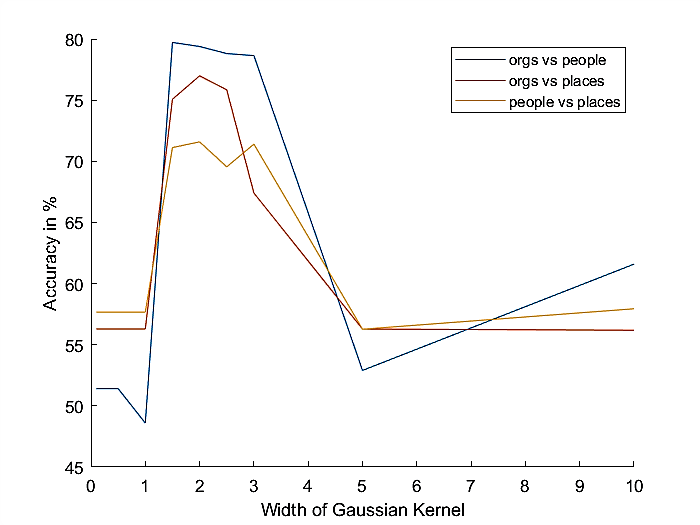
\includegraphics[width=\linewidth]{figures/PerformanceGaussianKernel.png}\label{FigPerfomanceTheta}}
\end{figure}
\FloatBarrier
\subsection{Theta Estimation}\label{InSubSecTheta}
Another, more deterministic but heuristic, approach to obtain a theta is presented by Kitayama in \cite{Kitayama.2011} and is discussed in the following.\\
It is important to notice that is just a simple estimation and therefore the optimal theta may not be found with this approach.\\
The width of the Gaussian kernel can play an important role not only for the \acs{PCVM} but many other algorithms.
Defining a 'good' value for the width leads to a more useful function which is observable in figure \ref{FigGaussianWidthRegression}.\cite{Kitayama.2011}
In this the black dots representing the data, the dashed lines are the Gaussian kernel, and the solid lines represent the regression.
In  \ref{FigSmallWidth} the width is set to 0.5 and in \ref{FigLargeWidth} it is set to 1.\newline
They are claiming in general that solving the theta via an optimisation problem is very time-consuming.
The reason for this is because the optimisation problem is depending on the data function, which can give a very large amount of variables and purposed a simpler algorithm to find a good $\theta$.\cite{Kitayama.2011}\\
First, they use a scaling technique to scale every dimension to an equal range.
Consider $N = N_\mathcal{Z} + N_\mathcal{X}$ as the number of all samples with $M$ dimensions.
In the approach, they using a \textit{Min-Max} Normalization to do it.\cite{Kitayama.2011}
\begin{equation}
	x_j = \frac{x_j - x_j^L}{x_j^U-x_j^L} \times s, \>\>\> i=1,\dots,M 
\end{equation}
Where $x_j^L$ is the lower bound and $x_j^U$ is the upper bound of value and $s=\alpha\times s \alpha \ge 0$.
The $s$ is the abort criterium, but not needed in our approach.
The author's recommendation is to set alpha to 1.1.
Moreover, therefore in every iteration of the algorithm, the dimension are rescaled.\\
However, in general, the training and test data for the \acs{PCVM} must be z-scored, as discussed in section \ref{Pc}.
Therefore it seems reasonable to replace the scaling technique from \textit{Min-Max} to the z-score:\cite{Mohamad.2013}.
\begin{equation}\label{EqZTrans}
x_{ij} = Z(x_{ij}) = \frac{x_{ij}-\mean{x}_j}{\sigma_j},\>\>\> i=1,\dots,N \>\>\> j=1,\dots,M
\end{equation}
Where $\mean{x}_j$ is the mean and $\sigma_j$ is the standard deviation in every dimension.\\
Furthermore, because after one run of z-score the mean is 0 and the standard deviation is 1.\cite{Mohamad.2013}
Revisiting \eqref{EqZTrans} with this, we obtain $x_{ij} = Z(x_{ij}) = \frac{x_{ij}}{1}$ after the first run, which is the same for every following iteration.
With this change, we omitted the need for further iteration and can calculate the width in one iteration.\\
After the z-score is applied, and the dimensions are equally scaled they originally continue with determining the distance.\cite{Kitayama.2011}
\begin{equation}\label{EqMaxDist}
	\theta_i = \frac{d_{i,max}}{\sqrt{N}\sqrt[N]{M-1}}, i=1,\dots,N
\end{equation}
Where $d_{j,max}$ is the maximum distance between the $i$-th data point and another data point.
And furthermore, $\theta_i$ is the width for the $i$-th Gaussian kernel in every row.\\
This is the main improvement in comparison with other approaches to determine the width because for example $\theta =\frac{d_{max}}{\sqrt[N]{NM}}$ can only be applied to uniform distributed data.
However with \eqref{EqMaxDist} the distance can be applied to non-uniform distributed data too, which is mostly the case in real-world problems.\cite{Kitayama.2011}\newline
Finally, we set our width to the smallest maximal distance found in \eqref{EqMaxDist}.
The estimate can be summarized in the following steps based on \cite{Kitayama.2011}:
\begin{enumerate}[label=\bfseries Step \arabic*:,leftmargin=*,labelindent=1em]
	\item Rescale data using z-score from \eqref{EqZTrans}
	\item Calculate the distance matrix
	\item Find maximum distance for $N$ data points using \eqref{EqMaxDist}
	\item Find the minimum distance for every training data with $\displaystyle\theta_{min}=\min_{1 \le i \le N}\theta_i$ and return $\theta_{min}$
\end{enumerate}
\begin{figure}
	\centering
	\begin{subfigure}{.5\textwidth}
		\centering
		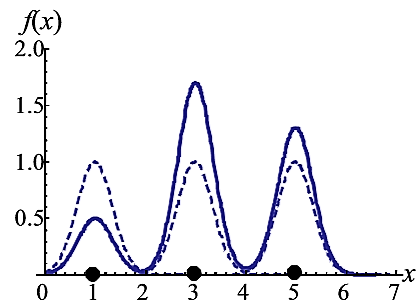
\includegraphics[width=1\linewidth]{figures/GaussianWidthSmall.png}
		\caption{Small Value \label{FigSmallWidth}}
	\end{subfigure}%
	\begin{subfigure}{.5\textwidth}
		\centering
		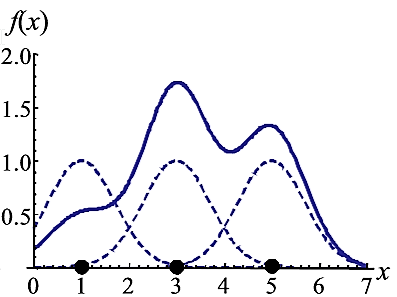
\includegraphics[width=1\linewidth]{figures/GaussianWidthLarge.png}
		\caption{Large Value \label{FigLargeWidth}}
	\end{subfigure}
	\caption[Effect of width in Gaussian Kernel]{Effect to regression of the width in the Gaussian kernel\cite{Kitayama.2011}}
	\label{FigGaussianWidthRegression}
\end{figure}
\FloatBarrier
To calculate the distance in practice, we are using a dissimilarity matrix D.
This matrix employs the euclidean distance with $d_{i,j}=||x_i-x_j||^2, \forall i,j \in N$ as dissimilarity measure.
This matrix is symmetric and is zero on the diagonal.\cite[p. 22,299]{Gentle.2007}\newline
Because the Gaussian kernel is used in this approach, the dissimilarity matrix is already involved in the computational complexity.
Furthermore, this matrix has just to be calculated once and can be reused in the theta estimation and the Gaussian kernel.
Another important thing to notice is that the data is already z-scored in the preparation and therefore there is no need to do it twice.
With this we just search the maximum distance with the built-in Matlab function \textit{min()} and can proceed with \eqref{EqMaxDist} in Step 3.
In the tests, we are using the whole dataset including training and testing.\\
Although we can reduce the complexity with a clever implementation, the complexity discussion is based on the worst case involving all steps to compute.
The computational complexity of calculating the dissimilarly matrix is $\mathcal{O}(N^2)$.\cite{Kobti.2007}
Furthermore, finding a maximum in $N$ rows with $M$ values can be solved in $\mathcal{O}(NM)$.
Because the dissimilarity matrix is symmetric the complexity changes to $\mathcal{O}(N^2)$ and multiplying a scalar to $N$ elements costs $\mathcal{O}(N)$, which can be summarised in $\mathcal{O}(N^2+N)=\mathcal{O}(N^2)$.
Again finding a minimum within the theta array from step 4 takes $\mathcal{O}(N)$.
Putting it together we can obtain the complexity of the theta estimation with $\mathcal{O}(N^2)$.
Note that in practice, we have no insight into the built-in Matlab function, which algorithm or implementation is used.
Because of this, the performance may be better for finding a minimum.
Furthermore, we observed for small datasets, that the theta would be large, which will eventually lead to a worse performance, see section \ref{EmSecDaDes} and table \ref{TableThetaEst}.
\subsection{Training Algorithm}\label{InSubSecTraining}
With the results from the previous section, \acs{PCTKVM} is presented in algorithm \ref{PseudoCodePCTKVM}.
\begin{algorithm}
	\caption{Probabilistic Classification Transfer Kernel Vector Machine }\label{PseudoCodePCTKVM}	
	\begin{algorithmic}[1]
		\Require Input Data $\mathbf{K} = [\mathbf{Z};\mathbf{X}]$ as $M$ sized training and $N$ sized text set; $\mathbf{Y}$ as $N$ sized training label vector; kernel(-type) \textit{ker}; eigenspectrum dumping factor $\zeta$; $\theta$ as kernel paramater; \textit{niter} as maximal number of iterations; \textit{threshold} as convergence criteria; \textbf{InitVector} as $M$-sized initialization vector.
		\Ensure Weight Vector $\mathbf{w}$; bias $b$, kernel parameter $\theta$; transfer kernel $\expP{\mathbf{K}}_\mathcal{A}$.
		\State $\mathbf{D}$ = calculate\_Dissimilarity\_Matrix($\mathbf{K}$);
		\State $\theta$ = theta\_Estimation($\mathbf{D}$);  \Comment{According to section \eqref{InSubSecTheta} (optional)}
		\State $\expP{\mathbf{K}}_\mathcal{A}$ = transfer\_Kernel\_Learning($\mathbf{D}$,\textit{ker},$\theta$,$\zeta$); \Comment{According to \eqref{InSecTrans}}
		\State [$\mathbf{w}$,$b$] = pcvm\_Training($\expP{\mathbf{K}}_\mathcal{Z}$,\textbf{InitVector},\textit{niter},\textit{threshold}); \Comment{Algorithm \eqref{PseudoCodePcvm}}
	\end{algorithmic}
\end{algorithm}
Note that the complete algorithm which involves every detail is found in appendix \ref{appac}. We observed in practice that the kernel is for some $\theta$ not \acs{PSD} anymore, although he is in theory.
We assume that there is some issue in the floating point multiplication for small numbers and therefore added the regularisation term $eps\mathbf{I}_{N\times N}$ to the kernel. 
This solved the problem.\\
As it can be seen the \acs{PCTKVM} the number of free parameters remains the same because the $\theta$ is estimated, only the eigenspectrum dumping factor $\zeta$ is left.
Furthermore, we obtain by combining the complexity of the theta estimation with \acs{PCVM} and \acs{TKL} the same complexity as already discussed, which is $\mathcal{O}(N_\mathcal{Z}^3+N_\mathcal{X}^2)$. The reason for this is that the dissimilarity matrix is already involved and can be validated in table \ref{TableMeanTimeRank}.
\subsection{Prediction}\label{InSubSecPrediction}
Additionally, we can make predictions based on the provided prediction function of the \acs{PCVM} with the use of $\expP{\mathbf{K}}_\mathcal{XZ} = \mathbf{U}_\mathcal{X}\mathbf{\Lambda}\expP{\mathbf{U}}_\mathcal{Z}^T$ as kernel.
When it comes to the \acs{SVM} the kernel has size $N_\mathcal{Z}\times N_\mathcal{X}$ is used for the prediction according to the support vectors.
The suggested prediction function for the \acs{SVM} has the form $\mathbf{y} = \expP{\mathbf{K}}_\mathcal{XZ}(\mathbf{\alpha}\odot\mathbf{y}_\mathbf{Z})+b$, where $\mathbf{\alpha}$ are the Lagrange multipliers.\cite{Long.2015}\newline
But because of the sparsity of the \acs{PCVM} the kernel size is greatly reduced as discussed in section \ref{Pc}.
If we consider that our model has $K$ non zero weight vectors with $K\ll N$ and because the \acs{PCVM} uses only kernel rows/columns corresponding to the non zero weight vector index, then our final kernel $\expP{\mathbf{K}}_\mathcal{KX}$ for prediction has size $(K\times N_\mathcal{X})$.
Therefore the prediction function of the \acs{PCTKVM} has the form:
\begin{equation}
\mathbf{y} = \expP{\mathbf{K}}_\mathcal{KX}\mathbf{w}+b
\end{equation}
Finally, the class label is obtained from the sign of the elements $y_i$ of the test label vector $\mathbf{y}_\mathcal{X}$ which has size $N_\mathcal{X}$.
The probabilistic output is calculated with the probit link function as the \acs{PCVM} does it in equation \ref{EqPcGausLike}.

\subsection{Extensions}\label{InSubSecExt}
In the course of this work, because the Image dataset has more than two classes, there was the need to implement a multi-class option for the \acs{PCVM}, \acs{PCTKVM} and \acs{PCTKVM}\textsubscript{$\theta$Est}.\\
To solve the multi-class problem algorithmically, there are two main approaches.
The first is the one vs rest approach.
Note that in the literature, the term one vs all appears instead of one vs rest.
If we consider $C$ classes, then the classifier would be trained with one class against the $C-1$ remaining classes.
This approach will have $C$ iteration, and in every iteration, another class is trained against each class.
The label assignment for one class is done in iteration only.
However, because this leads to large unclassifiable regions in the feature space.\cite[p. 114-116]{Abe.2010}\newline
Therefore the second approach, one vs one is implemented.
With this, we split up the labels in the different classes and train the classifier with every class against the others.
Again, if we take $C$, different classes, then our number of iteration is $K=C(C-1)/2$.
Furthermore, the unclassifiable region in comparison with the one vs rest approach is smaller.
At the predication we do again $K$ iteration and predict the whole dataset with two classes.\cite[p. 127-128]{Abe.2010}\newline
In the implementation consider a test set with size $N_\mathcal{X}$.
Then our label matrix $\mathbf{Y}$ and the probabilistic output matrix $\mathbf{P}$ has size $M\times K$.\\
We choose then the final label for the returning label vector $\mathbf{y}$ by counting the number of occurrences of a label for a data point.
The data point is then assigned to the label which the classifier has assigned the most.
In case of a tie the lower, the smaller class label is assigned regarding whole numbers, according to the Matlab \textit{mode}\footnote{https://de.mathworks.com/help/matlab/ref/mode.html} function.
This is rather unconventional because it is likely to be a random selection, but in our tests, the results are the best.
Another approach would be to assign the class label according to the biggest probability given from $\mathbf{P}$.\\
To determine a final probability output $\mathbf{p}$ for a final label decision with respect to the data point, the algorithm calculates the mean of the probabilistic output for the runs where the label is equal to the final label is assigned.\\
The number of relevance vectors is determined by using all unique vectors, which are used during the $K$ iterations.

\subsection{Further Extensions}\label{InSubSecFExt}
As suggested from \cite{Long.2015}, the current algorithm can be extended to multiple source learning.
With that, we can match the distribution difference of multiple source domains with the target domain.
This can be implemented by learning a $\mathbf{\Lambda}$ for every source/target combination and then using an existing multiple source learning, approach to predict the target based on multiple source domains.
For example, one could use the \ac{CP-MDA} algorithm from \cite{Chattopadhyay.2012} for it.\\
Another suggested extension is to adopt the algorithm to 'big data'.
Because kernel machine can have at least $\mathcal{O}(N^2)$ or even worse, they may not be applied well to very large datasets.
Here we can make use of the original Nyström method from \ref{InSecNysMeth} in combination with the Nyström Kernel approximation from \ref{InSubSecNyKerneLearning}.\cite{Long.2015}\\
Consider a large test kernel matrix $\mathbf{K}_\mathcal{X} \in \mathbb{R}^{N_\mathcal{X}\times N_\mathcal{X}}$.
Then sample from this kernel in a \acs{IID} manner to form a subset kernel $\mathbf{K}_\mathcal{X\hat{X}} \in \mathbb{R}^{N_\mathcal{X}\times \hat{N}_\mathcal{X}}$ with $\hat{N}_\mathcal{X} \ll N_\mathcal{X}$, which forms the subset $\mathcal{\hat{X}}$.
In the next step the eigensystem can be calculated through \eqref{EqEigsProb} and then the eigensystem of the target kernel can be extrapolated with:
\begin{equation}\label{EqLargeNsystromApprox}\cite{Long.2014}
	\mathbf{U}_\mathcal{X}=\mathbf{K}_\mathcal{X\hat{X}}\mathbf{U}_\mathcal{\hat{X}}\mathbf{\Lambda}_\mathcal{X}^{-1}
\end{equation}
Furthermore, we can approximate the source kernel $\mathbf{K}_{Z}$ with the  cross domain kernel $\mathbf{K}_{\mathcal{Z\hat{Z}}} \in \mathbb{R}^{N_\mathcal{Z}\times \hat{N_\mathcal{X}}}$ and the subset kernel $\mathbf{K}_\mathcal{\hat{Z}}$.
The procedure is similar to \eqref{EqLargeNsystromApprox} or with the use of the kernels only, shown in \eqref{EqTrainTestApprox} or \eqref{EqNystKernelApprox}, by replacing the target kernel with $\mathbf{K}_{\hat{Z}}$.
\begin{equation}
		\mathbf{K}_\mathcal{Z} \simeq	\mathbf{K}_{\mathcal{Z\hat{Z}}}\mathbf{K}_\mathcal{\hat{Z}}^{-1}\mathbf{K}_{\mathcal{\hat{Z}Z}}
\end{equation}
For being able to solve the quadratic programming problem from \eqref{EqTklQP}, we need to approximate the extrapolated eigensystem.
This means. First, we extrapolate the eigensystem of the target kernel to the source subset via \eqref{EqExtraEigs}:
\begin{equation}
\expP{\mathbf{U}}_\mathcal{\hat{Z}}\simeq\mathbf{K}_{\mathcal{\hat{Z}X}}\mathbf{U}_{\mathcal{X}}\boldsymbol{\Lambda}_\mathcal{\hat{X}}^{-1}
\end{equation}
Second, the approximated eigensystem has to be extrapolated to the full source data:
\begin{equation}
	\expP{\mathbf{U}}_\mathcal{Z} \simeq \mathbf{K}_{\mathcal{Z\hat{Z}}}\expP{\mathbf{U}}_\mathcal{\hat{Z}}\boldsymbol{\Lambda}_\mathcal{\hat{X}}^{-1}
\end{equation}
With this, we have the required information to solve the \acl{QP} and are making the \acs{TKL} algorithm large scale and applicable for big data.\cite{Long.2015}\\
Because it is a Nyström approximation, the quality of the approximation depends hardly on the quality of the taken sample, as mentioned in \ref{InSubSecNyKerneLearning}.
\section{Conclusion}\label{InSecCon}
In this chapter, we successfully integrated transfer learning in the \acs{PCVM}.
We successfully integrated a proposed transfer learning method in the \acs{PCVM}, which forms the \acs{PCTKVM}.
Furthermore, we solved the problem that the algorithm will be slow through the theta optimisation by adopting a simple theta estimation and adjust it to the needs of the \acs{PCVM}.
Because it uses unlabelled target data, the algorithm is transductive and solves the transfer problem with an relational-knowledge approach regarding homogeneous transfer learning.\\
Additionally, we extend the \acs{PCVM} and \acs{PCTKVM} to being able to solve multi-class problems via the one vs one approach.
The Matlab source code of the \acs{PCTKVM} and \acs{PCTKVM}\textsubscript{$\theta$Est} can be obtained from Github\footnote{https://github.com/ChristophRaab/pctkvm.git}.
Furthermore, the reader can find the complete code written for this thesis, including all tests, in the repository.
